% -----------------------------------------------------------------------------------------------%

% Oktober 2022
% Template Latex untuk Laporan Kerja Praktek Program Studi Sistem informasi ini
% Dikembangkan oleh Daffa Takratama Savra (daffatakratama13@gmail.com)

% Template ini dikembangkan dari template yang dibuat oleh Inggih Permana (inggihjava@gmail.com).

% Orang yang cerdas adalah orang yang paling banyak mengingat kematian.

% -----------------------------------------------------------------------------------------------%

% -----------------------------------------------------------------------------%
\chapter{\babDua}
% -----------------------------------------------------------------------------%
\section{Profil Instansi}
%-----------------------------------------------------------------------------%
\subsection{Sejarah}
%-----------------------------------------------------------------------------%
UIN Suska Riau memiliki fasilitas infrastruktur pendukung Tridharma Perguruan Tinggi yang baik, salah satunya adalah laboratorium terpadu di bawah Fakultas Sains dan Teknologi yang dikelola oleh Program Studi Sistem Informasi sejak tahun 2002. Terdapat tiga laboratorium yang dikelola oleh Program Studi Sistem Informasi, yaitu Laboratorium Rekayasa Sistem Informasi (RSI), Laboratorium Internet (INT), dan Laboratorium \textit{Software Engineering} (SE). Ketiga laboratorium tersebut merupakan aset penting yang dapat dimanfaatkan dengan baik untuk mencapai target-target universitas dan menghasilkan lulusan Program Studi Sistem Informasi yang kompeten dalam pendidikan, penelitian, serta pengabdian masyarakat dengan mengintegrasikan nilai-nilai keislaman. Laboratorium-laboratorium tersebut tidak hanya digunakan untuk praktikum mahasiswa sesuai dengan kurikulum, tetapi juga mampu mendukung berbagai kegiatan mahasiswa dan dosen dalam meningkatkan pengetahuan di bidang Sistem Informasi.
% -----------------------------------------------------------------------------%
\subsection{Visi}
% -----------------------------------------------------------------------------%
Menjadi laboratorium Program Studi Sistem Informasi yang memiliki keunggulan dalam bidang pendidikan, penelitian, dan pengabdian kepada masyarakat dengan menghasilkan lulusan yang proaktif, inovatif, dan profesional dalam bidang Sistem Informasi di tingkat lokal, regional, dan nasional yang berbasis nilai-nilai islami pada tahun 2030.
% -----------------------------------------------------------------------------
\subsection{Misi}
% -----------------------------------------------------------------------------%
Untuk mencapai Visi Laboratorium Program Studi Sistem Informasi, berikut Misi-misi yang harus dicapai, diantaranya:

\begin{enumerate}

  \item Mendukung penyelenggaraan kegiatan pendidikan akademik dan praktikum berbasis teknologi kepada mahasiswa, dosen, dan stakeholder.
  \item Mendukung pelaksanaan kegiatan penelitian yang berbasis teknologi kepada mahasiswa, dosen, dan stakeholder.
  \item Mendukung kegiatan pengabdian kepada masyarakat yang berbasis teknologi.
  \item Menyiapkan sumber daya manusia yang mampu menerapkan teknologi informasi khususnya dibidang Sistem Informasi.
  \item Membangun kemitraan dan jejaring dengan industri, pemerintah, dan organisasi nasional.

\end{enumerate}
% -----------------------------------------------------------------------------%
\subsection{Struktur Organisasi}
% -----------------------------------------------------------------------------%
Untuk menjalankan Tridharma Perguruan Tinggi dengan baik, pengelola laboratorium harus memiliki kemampuan manajerial yang baik dan dibantu dengan keahlian IT. Untuk mencapai hal ini, diperlukan sekelompok pengelola laboratorium yang percaya diri dan memiliki kemampuan. Gambar 2.1 menunjukkan struktur organisasi pengelola laboratorium Program Studi Sistem Informasi dari 2021 hingga 2024.

\begin{figure}
  \centering
  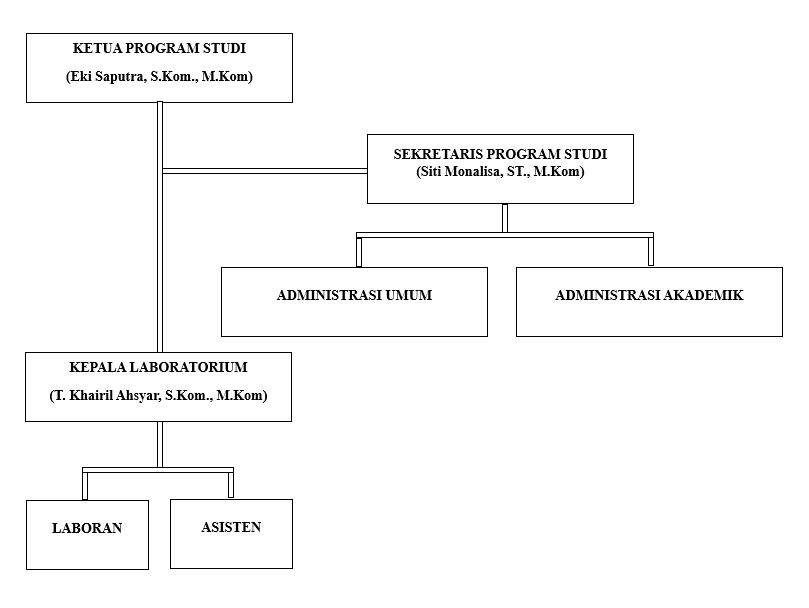
\includegraphics[width=0.82\linewidth]{konten//gambar/Struktur Organisasi.png}
  \caption{Struktur Organisasi Laboratorium}
  \label{fig:enter-label}
\end{figure}
% \subsection{a}
% % -----------------------------------------------------------------------------%
% \subsection{a}
% % -----------------------------------------------------------------------------%
% \begin{enumerate}
% 	\item Isi sesuai keinginan
% \end{enumerate}
% % -----------------------------------------------------------------------------%
% \section{Sistem}
% % -----------------------------------------------------------------------------%
% Sistem adalah suatu jaringan kerja dari prosedur-prosedur yang saling berhubungan, berkumpul bersama-sama untuk melakukan suatu kegiatan atau menyelesaikan suatu sasaran tertentu (Ahmad dan Hasti, 2018). Sistem juga bisa diartikan sebagai kesatuan bagian-bagian yang saling berhubungan yang berada dalam suatu wilayah serta memiliki item-item penggerak, dan bisa diartikan menjadi sangat luas, pada bidang computer fungsi sistem tersebut dapat berupa media untuk melakukan input, proses, dan output (hasil) dari suatu data \cite{audrilia2020perancangan}
% -----------------------------------------------------------------------------%
% \section{Informasi}
% Informasi merupakan hasil dari pengolahan data sehingga menjadi bentuk yang penting bagi penerimanya dan mempunyai kegunaan sebagai dasar dalam pengambilan keputusan yang dapat dirasakan akibatnya secara langsung saat itu juga atau secara tidak langsung pada saat mendatang \cite{henny2020sistem}. Dalam arti lain informasi adalah data yang diolah menjadi bentuk yang lebih berguna berarti bagi penggunanya \cite{audrilia2020perancangan}
% -----------------------------------------------------------------------------%

\section{Inventaris}
Inventaris merupakan sebuah kata yang diasimilasikan dari kata \textit{inventory} yang berasal dari bahasa Inggris. Echols dan Shadily merumuskan dalam kamus Besar Bahasa Indonesia sebagai daftar barang disertai dengan nilainya masing-masing yang dimilki perusahaan dalam kurun waktu tertentu yang digunakan dalam kegiatan usaha perusahaan. Dalam praktek, inventaris disebut juga sebagai persediaan barang yang artinya barang-barang biasanya dapat dijumpai digudang tertutup, lapangan, gudang terbuka atau tempat-tempat penyimpanan lain, baik berupa bahan baku, barang setengah jadi, barang jadi barang-barang untuk keperluan operasi atau barang-barang untuk keperluan suatu proyek \cite{novendri2019aplikasi}.
% -----------------------------------------------------------------------------%
\section{Sistem Informasi Inventaris}
% -----------------------------------------------------------------------------%
Sistem informasi adalah suatu sistem didalam Organisasi yang mempertemukan kebutuhan pengolahan transaksi harian, mendukung operasi bersifat manajerial dan kegiatan strategi dari suatu organisasi dan menyediakan pihak luar tertentu dengan laporan-laporan yang diperlukan \cite{laila2011sistem}. Sistem informasi inventaris adalah suatu sistem yang digunakan untuk mengelola dan memantau inventaris atau barang yang dimiliki oleh suatu organisasi atau perusahaan. Sistem ini dapat membantu memudahkan petugas inventaris dalam pendataan barang yang dimiliki oleh organisasi atau perusahaan tersebut \cite{Yanti2021SISTEMII}.
%-----------------------------------------------------------------------------%
%-----------------------------------------------------------------------------%
\section{Laboratorium}
Laboratorium merupakan sarana dalam melaksanakan sebuah riset dalam bidang ilmiah, eksperimen, pengukuran maupun pelatihan ilmiah. Meski laboratorium telah memiliki alat-alat yang lengkap, pengelolaan laboratorium juga harus diperhatikan. Adanya alat-alat yang sudah lengkap dan penggunaan yang sudah baik tentunya perlu untuk dilakukan manajemen yang baik pada laboratorium tersebut, karena terdapat beberapa hal yang harus diperhatikan kembali seperti pengelolaan masing-masing laboratorium dan pengolahan data \cite{sweden2022rancang}.
\subsection{Laboratorium Rekayasa Sistem Informasi (RSI)}
Laboratorium Rekayasa sistem Informasi atau yang disingkat dengan nama Laboratorium RSI merupakan laboratorium pertama yang dimiliki oleh Program Studi Sistem Informasi sejak pindahnya aktivitas perkuliahan kampus dari kampus Sukajadi ke kampus utama Panam Pekanbaru Riau pada tahun 2007. Fungsi utama dari laboratorium ini adalah sebagai fasilitas infrastruktur pendukung untuk pelaksanaan kegiatan perkuliahan praktikum bagi mahasiswa Program Studi Sistem Informasi terkait bidang Rekayasa Sistem Informasi. Bidang Rekayasa Sistem Informasi merupakan bidang yang paling dominan yang ada di Program Studi Sistem Informasi \cite{lab-si-website}.

\subsection{Laboratorium Internet (INT)}
Laboratorium Internet atau yang disingkat dengan nama Laboratorium INT merupakan laboratorium milik Program Studi Sistem Informasi di bawah Fakultas Sains dan Teknologi kedua yang aktivitas perkuliahannya berada di kampus utama Panam Pekanbaru Riau. Secara spesifik, laboratorium ini lebih dioperasikan untuk kebutuhan perkuliahan terkait matakuliah praktikum dasar, seperti matakuliah Jaringan Komputer dan Pemrograman Dasar \cite{lab-si-website}.

\subsection{Laboratorium \textit{Software Engineering} (SE)}
Laboratorium ke tiga yang dimiliki oleh Program Studi Sistem Informasi adalah Laboratorium \textit{Software Engineering} atau yang disingkat dengan nama Laboratorium SE. Laboratorium ini merupakan laboratorium terbaru milik yang dikelola oleh Program Studi dari usulan pengadaan barang tahun anggaran 2021 di bawah naungan Fakultas Sains dan Teknologi UIN Suska Riau. Adapun laboratorium SE sebagai pendukung dalam pelaksanaan kegiatan perkuliahan praktikum bagi mahasiswa Program Studi Sistem Informasi yang terkait dengan bidang keilmuan seperti Praktikum Basis Data, Pemrograman Beorientasi Objek (PBO), dan matakuliah wajib praktikum lainnya \cite{lab-si-website}.

%-----------------------------------------------------------------------------%
\section{Web}
Rangkaian jaringan yang tersebar di seluruh dunia, yang di semua organisasi dihubungkan oleh jaringan terbesar sehingga dapat saling berkomunikasi, adalah istilah internet. Dengan Internet, pengguna dapat mengakses berbagai sistem dari mana saja, internet juga sebagai penghubung jaringan website. \textit{World Wide Web} (WWW) atau Website adalah laman-laman berisikan keterangan yang berada dalam taraf global berbasis \textit{hypertext} yang memungkinkan pengguna mencari banyak sekali macam keterangan pada dunia selama terhubung menggunakan internet \cite{tyowati2017implementasi}.
%-----------------------------------------------------------------------------%
\section{\textit{Framework}}
\textit{Framework} dalam pengembangan sistem adalah kerangka kerja atau struktur yang digunakan untuk memudahkan pengembangan aplikasi atau sistem \cite{sallaby2020perancangan}. \textit{Framework} menyediakan berbagai fitur dan fungsi yang dapat digunakan oleh pengembang untuk mempercepat proses pengembangan dan memastikan konsistensi dalam pengembangan aplikasi atau sistem \cite{simanullang2021sistem}. \textit{Framework} juga membantu pengembang dalam mengelola kode program dan memperbaiki bug. Beberapa contoh \textit{framework} yang sering digunakan dalam pengembangan sistem adalah Laravel, CodeIgniter, dan beberapa \textit{framework} lainnya \cite{Fadllullah2022PengembanganSI}.
%-----------------------------------------------------------------------------%
\section{Codeigniter}
Codeigniter merupakan \textit{framework} untuk membangun aplikasi web berbasis PHP  Codeigniter menyediakan banyak \textit{library} untuk fungsi-fungsi umum, antar muka yang sederhana, dan struktur yang logis. CodeIgniter menjadi sebuah \textit{framework} PHP dengan model MVC \textit{(Model, View, Controller)} untuk membangun website dinamis dengan menggunakan PHP yang dapat mempercepat pengembang untuk membuat sebuah aplikasi web. Selain ringan dan cepat, CodeIgniter juga memiliki dokumentasi yang super lengkap disertai dengan contoh implementasi kodenya. Programmer dapat membuat aplikasi dengan lebih cepat karena tidak perlu menulis kode dari awal, selain itu Codeigniter juga menyediakan banyak fungsi yang siap digunakan. Seorang programmer bisa lebih fokus dengan aplikasi yang sedang dibangun dan meminimalkan penulisan kode \cite{tyowati2017implementasi}.
%-----------------------------------------------------------------------------%
\section{\textit{Database}}
\textit{Database} adalah suatu kumpulan data yang telah diatur secara terstruktur, memungkinkan akses dan pengelolaan melalui sistem komputer. Jenis data yang dapat disimpan di dalamnya mencakup teks, gambar, suara, dan video, dengan berbagai tujuan seperti penyimpanan informasi, analisis data, dan pengambilan keputusan. Untuk membuat dan mengelola \textit{database}, diperlukan perangkat lunak khusus seperti MariaDB, Oracle, atau Microsoft SQL Server \cite{Cowls2021ADB}.
%-----------------------------------------------------------------------------%
\section{MariaDB}
MariaDB sebenarnya merupakan turunan salah satu konsep utama dalam basis data yang telah ada sebelumnya SQL \textit{(Structured Query Language)}. SQL adalah sebuah konsep pengoperasian basis data, terutama untuk pemilihan atau seleksi dan pemasukan data yang memungkinkan pengoperasian data dikerjakan dengan mudah secara otomatis \cite{priyanti2013sistem}.
%-----------------------------------------------------------------------------%
\section{PHP}
\textit{Hypertext Preprocessor} (PHP) adalah pemrograman interpreter yaitu proses penerjemahan baris kode sumber menjadi kode mesin yang dimengerti komputer secara langsung pada saat baris kode dijalankan. PHP disebut sebagai pemrograman \textit{Server Side Programming}, hal ini dikarenakan seluruh proses nya dijalankan pada server. PHP adalah sebuah bahasa dengan hak cipta terbuka atau yang juga dikenal dengan istilah \textit{open source}, yaitu pengguna dapat mengembangkan kode-kode fungsi PHP sesuai dengan kebutuhannya \cite{php2001php}.
%-----------------------------------------------------------------------------%
\section{XAMPP}
XAMPP adalah sebuah paket lengkap untuk server web yang dapat dengan mudah diinstal di berbagai sistem operasi. Dalam paket ini sudah termasuk beberapa komponen penting seperti Apache (web server), MariaDB \textit{(database)}, PHP (server side scripting), dan berbagai pustaka pendukung lainnya. XAMPP dapat digunakan pada berbagai sistem operasi, termasuk Linux, Windows, MacOS, dan Solaris, sehingga memudahkan pembuatan server web \textit{multi-platform} \cite{pakpahan2020sistem}.
%-----------------------------------------------------------------------------%